\documentclass[../main]{subfiles}

\begin{document}

\section{Subgradient method}\label{subgradient-method}

To solve the reduced problem for $\lambda$, we consider a class of subgradient
methods:

\begin{equation}\lambda_{k+1} = \mathbf{P}(\lambda_{k} + s_{k}d_{k})\end{equation}

where \(\mathbf P\) is the projection onto dual space \(\Lambda\).
\(d_k\) is the update direction for current iteration and \(s_{k}\) is
the step size using target-based rule:

\begin{equation}\label{eq:step_size}
  s_{k} = \gamma_k\frac{\phi^\star - \phi(\lambda_k)}{||d_{k}||^2}
\end{equation}

Note the direction \(d_k\) computed by

\begin{equation}\label{eq:direction}
  d_k = \bar y_k - b
\end{equation}

where \(\bar y_k\) is the convex combination of previous iterations
\(\{y_i\}_{i=1,...k}\) and each \(y_i\) solves
\(\phi_i = \phi(\lambda_i)\):

\begin{equation}\bar y_k = \sum^i_k \alpha^i_k y_i,\quad  \sum^i_k \alpha^i_k = 1, \alpha^i_k \ge 0\end{equation}

Alternatively, one can express the convexity in a recursive manner:

\begin{equation}\bar y_k = (1-\alpha_k)\cdot\bar y_{k-1} + \alpha_k \cdot y_k \end{equation}

For we simplicity take \(g_k= y_k - b\), then \(g_k\) is a subgradient
of \(\phi\) at \(\lambda_k\):

\begin{equation}g_k \in \partial \phi_k\end{equation}

The direction can be rewritten as the combination of the subgradient and
previous directions:

\begin{equation}\label{eq:direction_recursive}
  d_k = (1-\alpha_k) \cdot d_{k-1} + \alpha_k\cdot g_k
\end{equation}


The dual subgradient algorithm can be summarized as follows.
\(\varepsilon,\varepsilon_s\) are the tolerance parameter for objective gap and stepsize, respectively.
\(\varepsilon > 0 ,\varepsilon_s > 0\).

\begin{algorithm}[H]
  \SetAlgoLined
  Initialization. \(\alpha_0 = 1, \lambda_0 = e, \gamma_0 = 1\)  \\
  \While{\(\bar z_k - \phi_k \ge \varepsilon\) \textbf{and} \(s_k \ge \varepsilon_s\)}
  {
    Let current iteration be \(k\)\\
    Update the multipliers by
    \[\lambda_{k} = \mathbf{P}(\lambda_{k-1} + s_{k-1}d_{k-1})\]

    Solve dual problem \(\phi_k\) by \eqref{eq:dual}
    and compute subgradient \(g_k\) respectively.

    Compute \(\gamma_k, \alpha_k\) properly.

    Compute current direction by \eqref{eq:direction} or \eqref{eq:direction_recursive}

    Update \(\epsilon_k,\delta_k ,\bar \epsilon_k ,\bar \delta_k, z_k, \bar z_k \)
    by the \underline{Recovery Algorithm} \ref{alg:recovery}

    Stepsize is updated by \eqref{eq:step_size}
  }
  \caption{The Subgradient Algorithm}
\end{algorithm}

It is obvious to see the solutions during dual optimization
\((y, \epsilon, \delta) = (y_k, 0, 0)\) are feasible if and only if we
can find \(y_k = d\), which in general will not hold. This motivates the following
algorithm based on linear programming theory.

\begin{algorithm}[H]\label{alg:recovery}
  \SetAlgoLined
  \begin{equation}\label{eq:recovery}
    \begin{aligned}
       & \epsilon_k = \max\{y_k - b, 0\}           \\
       & \delta_k = \max\{b - y_k, 0\}             \\
       & \bar \epsilon_k = \max\{\bar y_k - b, 0\} \\
       & \bar \delta_k = \max\{b - \bar y_k, 0\}
    \end{aligned}\end{equation}
  \caption{Recovery Algorithm}
\end{algorithm}

To simplify our presentation, let
\(z\) be a function of \(y\) such that \(z_k = z(y_k) = f(\delta_k, \epsilon_k)\), then \(z\) is
also convex in \(y\) since both function \(f\) and \(\max\{\cdot, 0\}\)
are convex. It's also worth to notice that \(\bar \epsilon_k\) should
not be calculated as running averages:
\(\bar \epsilon_k \neq \sum^i_k \alpha^i_k \epsilon_i\). For such an
``averaged'' solution, we let
\(\bar z_k = z(\bar y_k)\). We later find the recovery algorithm achieves
at the optimal objective.



\section{Convergence}\label{convergence}


We first review several features for the subgradient method regarding
parameters \(\gamma_k, \alpha_k\) and search direction \(d_k\) produced from convex combinations.

The target based rule are well-known as the Polyak rule \cite{polyak_general_1967}.
The idea of using previous searching directions is introduced to accelerate the subgradient method and provide a better stopping criterion,
see \cite{camerini1975improving}, \cite{brannlund1995generalized}, \cite{barahona_volume_2000}.
\cite{brannlund1995generalized} showed that with convex combinations the optimal choice of stepsize is
equivalent to the Camerini-Fratta-Maffioli modification, it also provides an analysis on its linear convergence rate.

From the primal perspective, our method is close to \emph{primal
  averaging method}. \cite{nedic_approximate_2009}
gives a line of analysis on convergence and quality of the primal
approximation by averaging over all previous solutions with a constant
stepsize. They use a simple averaging scheme that can be rephrased into a
recursive equation with \(\alpha_k = 1/k\) such that:

\[\bar y_k = \frac{k-1}{k}\cdot\bar y_{k-1} + \frac{1}{k} \cdot y_k\]

then it gives lower and upper bounds for the averaged solution
that involve the primal violation, norm of the subgradient, etc. Furthermore, they only analyze the case for constant
stepsize \(s_k = s, s\ge 0\) and the search direction defined solely by
the subgradient. We refer to \cite{kiwiel_lagrangian_2007} for target based
stepsizes. The volume algorithm proposed by \cite{barahona_volume_2000} is close to the
case mentioned in \cite{brannlund1995generalized} in a dual
viewpoint while adopting \(\hat \lambda_{k}\) instead of \(\lambda_k\) from the best dual bound
\(\hat \phi_k = \max_{i=1, ..., k} \phi(\lambda_i)\):

\[\lambda_{k+1} = \mathbf{P}(\hat\lambda_{k} + s_{k}d_{k})\]

\emph{There is no existing proof of convergence} for the volume
algorithm.

\textbf{(Remark / Difference for our method)}

Since the solution is strictly feasible by implementation of the
recovery algorithm \ref{eq:recovery}, i.e., there is no need to bound for feasibility gap
as has been done in most of literature covering the \textbf{primal
  recovery}. Instead, we have analyze the quality of the heuristic, i.e.:

\[
  |\bar z_k - \phi_k| \textrm { or } |\bar z_k - z^\star|
\]

We found its convergence is closely related to strong duality of the problem. Accounting for performance,
we suggest several specific choices of parameters regarding the subgradient method \((\gamma, \alpha, d)\).


\subsection{Analysis outline}\label{analysis-outline}

\begin{itemize}

  \item
        we've showed \(\phi^\star = f^\star= z^\star\)
  \item
        we show \(\lambda_k\) converges to \(\lambda^\star \in \Lambda^\star\)
        for our choices of \(\gamma_k, \alpha_k\)
  \item
        we show primal solution \(\bar z_k\) converges to \(z^\star\)
\end{itemize}

\begin{lemma}\(\epsilon\)-subgradient.
  \begin{equation}\label{eq:subgrad}
    \begin{aligned}
      g_{k}^\mathsf{T}(\lambda_{k}  -\lambda) \le \phi_{k} - \phi(\lambda) \\
      d_{k}^\mathsf{T}(\lambda_{k}  -\lambda) \le \phi_{k} - \phi(\lambda) + \epsilon_k
    \end{aligned}
  \end{equation}
\end{lemma}

where

\begin{equation}\label{eq:def_eps}
  \epsilon_k = \sum^i_k \alpha^i_k \cdot \left [g_i^\mathsf{T}(\lambda_k - \lambda_i) + \phi_i - \phi_k \right ]
\end{equation}

Notice \(\epsilon_k\) can be further simplified by the definition of
\(\phi\):

\begin{equation}\label{eq:def_eps_simple}
  \epsilon_k = \sum^i_k \alpha^i_k \cdot \left ( g_i^\mathsf{T}\lambda_k  - \phi_k \right )
\end{equation}

\begin{lemma} \label{lemma:dual_conv} Dual convergence, \cite{brannlund1995generalized}. The
  subgradient method is convergent if \(\epsilon_k\) satisfies:
  \begin{equation}
    \frac{1}{2}(2 - \gamma_k) (\phi_{k} - \phi^\star)  + \epsilon_k \le 0
  \end{equation}
\end{lemma}
\begin{proof}
  The proof can be done by showing the monotonic decrease of
  \(\|\lambda_{k} - \lambda^\star\|\) via the iterative equations.
  \begin{equation}\begin{aligned}
      \|\lambda_{k+1} - \lambda^\star\|^2 \le ||\lambda_k - \lambda^\star||^2
      + 2\cdot \gamma_k \frac{(\phi^\star - \phi_{k})}{\|d_{k}\|^{2}} d_k^\mathsf{T}(\lambda_k - \lambda^\star)
      + (\gamma_{k})^{2} \frac{(\phi^\star - \phi_{k})^{2}}{\|d_{k}\|^{2}}
    \end{aligned}\end{equation}

  Notice: \begin{equation}\begin{aligned}
          & 2  \cdot d_k^\mathsf{T}(\lambda_k - \lambda^\star) + \gamma_{k}(\phi^\star - \phi_{k})
      \le & 2 (\phi_{k} - \phi^\star + \epsilon_k) + \gamma_k(\phi^\star -\phi_k)                  \\
      =   & (2 - \gamma_k) (\phi_{k} - \phi^\star)  + 2\epsilon_k \le 0
    \end{aligned}\end{equation}

  and we have the convergence.
\end{proof}

\begin{theorem} \label{lemma:recovery}  Recovery Algorithm \eqref{eq:recovery}
  \begin{enumerate}
    \def\labelenumi{(\alph{enumi})}

    \item
          For fixed \(y=y_k\), \((\epsilon_k, \delta_k)\) is the optimal
          solution for the restricted primal problem.
  \end{enumerate}

  \[f(\epsilon_k, \delta_k) \le f(\epsilon, \delta), \quad \forall \delta\ge 0, \epsilon\ge 0, y= y_k\]

  \begin{enumerate}
    \def\labelenumi{(\alph{enumi})}
    \setcounter{enumi}{1}

    \item
  \end{enumerate}

  \[\bar z_k \le \sum^i_k \alpha^i_k z^i\]
  \begin{enumerate}
    \def\labelenumi{(\alph{enumi})}
    \setcounter{enumi}{2}

    \item
  \end{enumerate}
  \[\bar z_k \ge d_k^\mathsf{T} \lambda_k\]

\end{theorem}

\begin{proof}
  (a) straight-forward. (b) by convexity of \(z(\cdot)\). (c)
  we notice a strong duality pair with fixed \(d_k\) at each iteration
  \(k\).

  \begin{equation}
    \begin{aligned}
      \mathbf{(P)}  \quad & \min_{\delta, \epsilon} p^\mathsf{T} \delta + h^\mathsf{T} \epsilon \\
      \mathbf{s.t.} \quad & d_k + \delta - \epsilon = 0                                         \\
                          & \delta \in \mathbb{R}_+^n, \epsilon \in \mathbb{R}_+^n
    \end{aligned}
  \end{equation}

  and

  \begin{equation}
    \begin{aligned}
      \mathbf{(D)}  \quad & \max_{\lambda} d_k^\mathsf{T} \lambda          \\
      \mathbf{s.t.} \quad & -p \le \lambda \le h, \lambda \in \mathbb{R}^n
    \end{aligned}
  \end{equation}

  by \ref{lemma:recovery}(a), \((\bar \epsilon_k, \bar \delta_k)\) minimizes the primal
  problem. Since \textbf{(P)} is well-defined,
  \(\exists\; \mu_k \in [-p, h]\) such that \(\mu_k \in \arg\max_{\lambda} d_k^\mathsf{T} \lambda \).

  \[\begin{aligned}
       & d_k^\mathsf{T} \mu_k = \bar z_k = p^\mathsf{T} \bar \delta_k + h^\mathsf{T} \bar \epsilon_k \\
       & d_k^\mathsf{T} \mu_k \ge  d_k^\mathsf{T} \lambda_k
    \end{aligned}\]


\end{proof}

Now we visit properties for primal solutions.

\begin{theorem} \label{theorem:primal}

  Suppose the subgradient is bounded, that is, \(\exists L > 0\) such that

  \begin{equation}\label{eq:bounded_subgrad}
    \|g_k\| \le L
  \end{equation}

  and
  \begin{equation}\label{eq:non_orthogonal_direction}
    d_k^\mathsf{T} d_{k+1} \ge 0
  \end{equation}
  holds for all iteration \(k\) in the subgradient algorithm.
  Then the primal-dual bound by the recovery algorithm \eqref{eq:recovery} converges to \(0\), specifically:

  \[\bar z_k - \phi^\star \to 0\]

\end{theorem}

\begin{proof}
  We first notice

  \[
    \phi^\star - \phi_k \le g_k^\mathsf{T} (\lambda^\star - \lambda_k)\le \|g_k\|\|\lambda^\star - \lambda_k\| \Rightarrow \phi_k -\phi^\star
  \]

  This immediately follows:
  \begin{subequations}
    \begin{align}\label{eq:eps_subgrad_to_subgrad}
                        & \epsilon_k \le \frac{1}{2}(2 - \gamma_k) ( \phi^\star - \phi_k) \to 0 \\
      \Rightarrow \quad & \epsilon_k = d_k^\mathsf{T} \lambda_k - \phi_k \to 0                  \\
      \Rightarrow \quad & d_k^\mathsf{T} \lambda_k \to \phi^\star
    \end{align}
  \end{subequations}

  We now show the convergence from \(\bar z\) to \(\lambda_k ^ \mathsf{T} d_k\).

  % \begin{equation}
  %   \begin{aligned}\label{eq:bar_z_to_lambda_d}
  %     \bar z_{k+1} - \lambda_{k+1}^\mathsf{T} d_{k+1}
  %      & = z\left(\alpha g_k + (1-\alpha) d_k\right) - (\lambda_k + s_k d_k ) \left ((1-\alpha) d_k + \alpha g_k \right ) \\
  %      & \le \alpha \cdot z(g_k) + (1-\alpha) \cdot z(d_k)
  %     - (1-\alpha)\lambda_k^\mathsf{T} d_k - (1-\alpha) s_k \|d_k\|^2
  %     - \alpha \lambda_k ^\mathsf{T} g_k - \alpha s_k d_k^\mathsf{T} g_k                                                  \\
  %      & = (1-\alpha)(\bar z_k - \lambda_k ^ \mathsf{T} d_k) - s_k d_k \Big [ \alpha  g_k + (1-\alpha) d_k \Big]          \\
  %      & = (1-\alpha)(\bar z_k - \lambda_k ^ \mathsf{T} d_k) - s_k d_k^\mathsf{T} d_{k+1}                                 \\
  %      & \le (1-\alpha)(\bar z_k - \lambda_k ^ \mathsf{T} d_k)
  %   \end{aligned}
  % \end{equation}

  % We combine \eqref{eq:bar_z_to_lambda_d}, \eqref{eq:eps_subgrad_to_subgrad} to $\bar z^k \to \phi^\star$
\end{proof}

% \emph{Remark}

% The boundedness of subgradient can be easily verified by \eqref{eq:direction}. As for \eqref{eq:non_orthogonal_direction},
% \cite{brannlund1995generalized} suggests the orthogonality \(d_k^\mathsf{T} d_{k+1} = 0\) if the optimal stepsize is implemented.
% Our results show that the angle between two consecutive search directions should be acute to achieve better duality gaps.


The next proposition states several convergence-guaranteed choices on
parameters for convexity \(\alpha_k\) and stepsize \(\gamma_k\). Part
(a) originally appears in \cite{brannlund1995generalized}. Besides, we
also consider a slower scheme that is widely used and simple to
implement.


\begin{corollary} Choices of parameters. to show the following is convergent?

  \[\alpha_k = \frac{1}{k}, \gamma_k = \gamma \in [1, 2]\]

\end{corollary}


\subsection{Computational Results}\label{computational-results}

We present our computational results to validate the convergence analysis on subgradient method
as shown in Figure \ref{fig:divergent_volume}.
The experiments are done on the Fleet Maintenance Problem.
Our results show that averaged solution by recovery algorithm \eqref{eq:recovery} converges to the best lower bound.
The baseline is set by MILP modeled in Gurobi 9.1 to provide lower bound and best integral solution.
We implement subgradient methods mentioned in our paper in Python 3.7. Specifically, ...

\begin{figure}
  \subfloat[][Normal subgradient method using \(g_k\)]{
    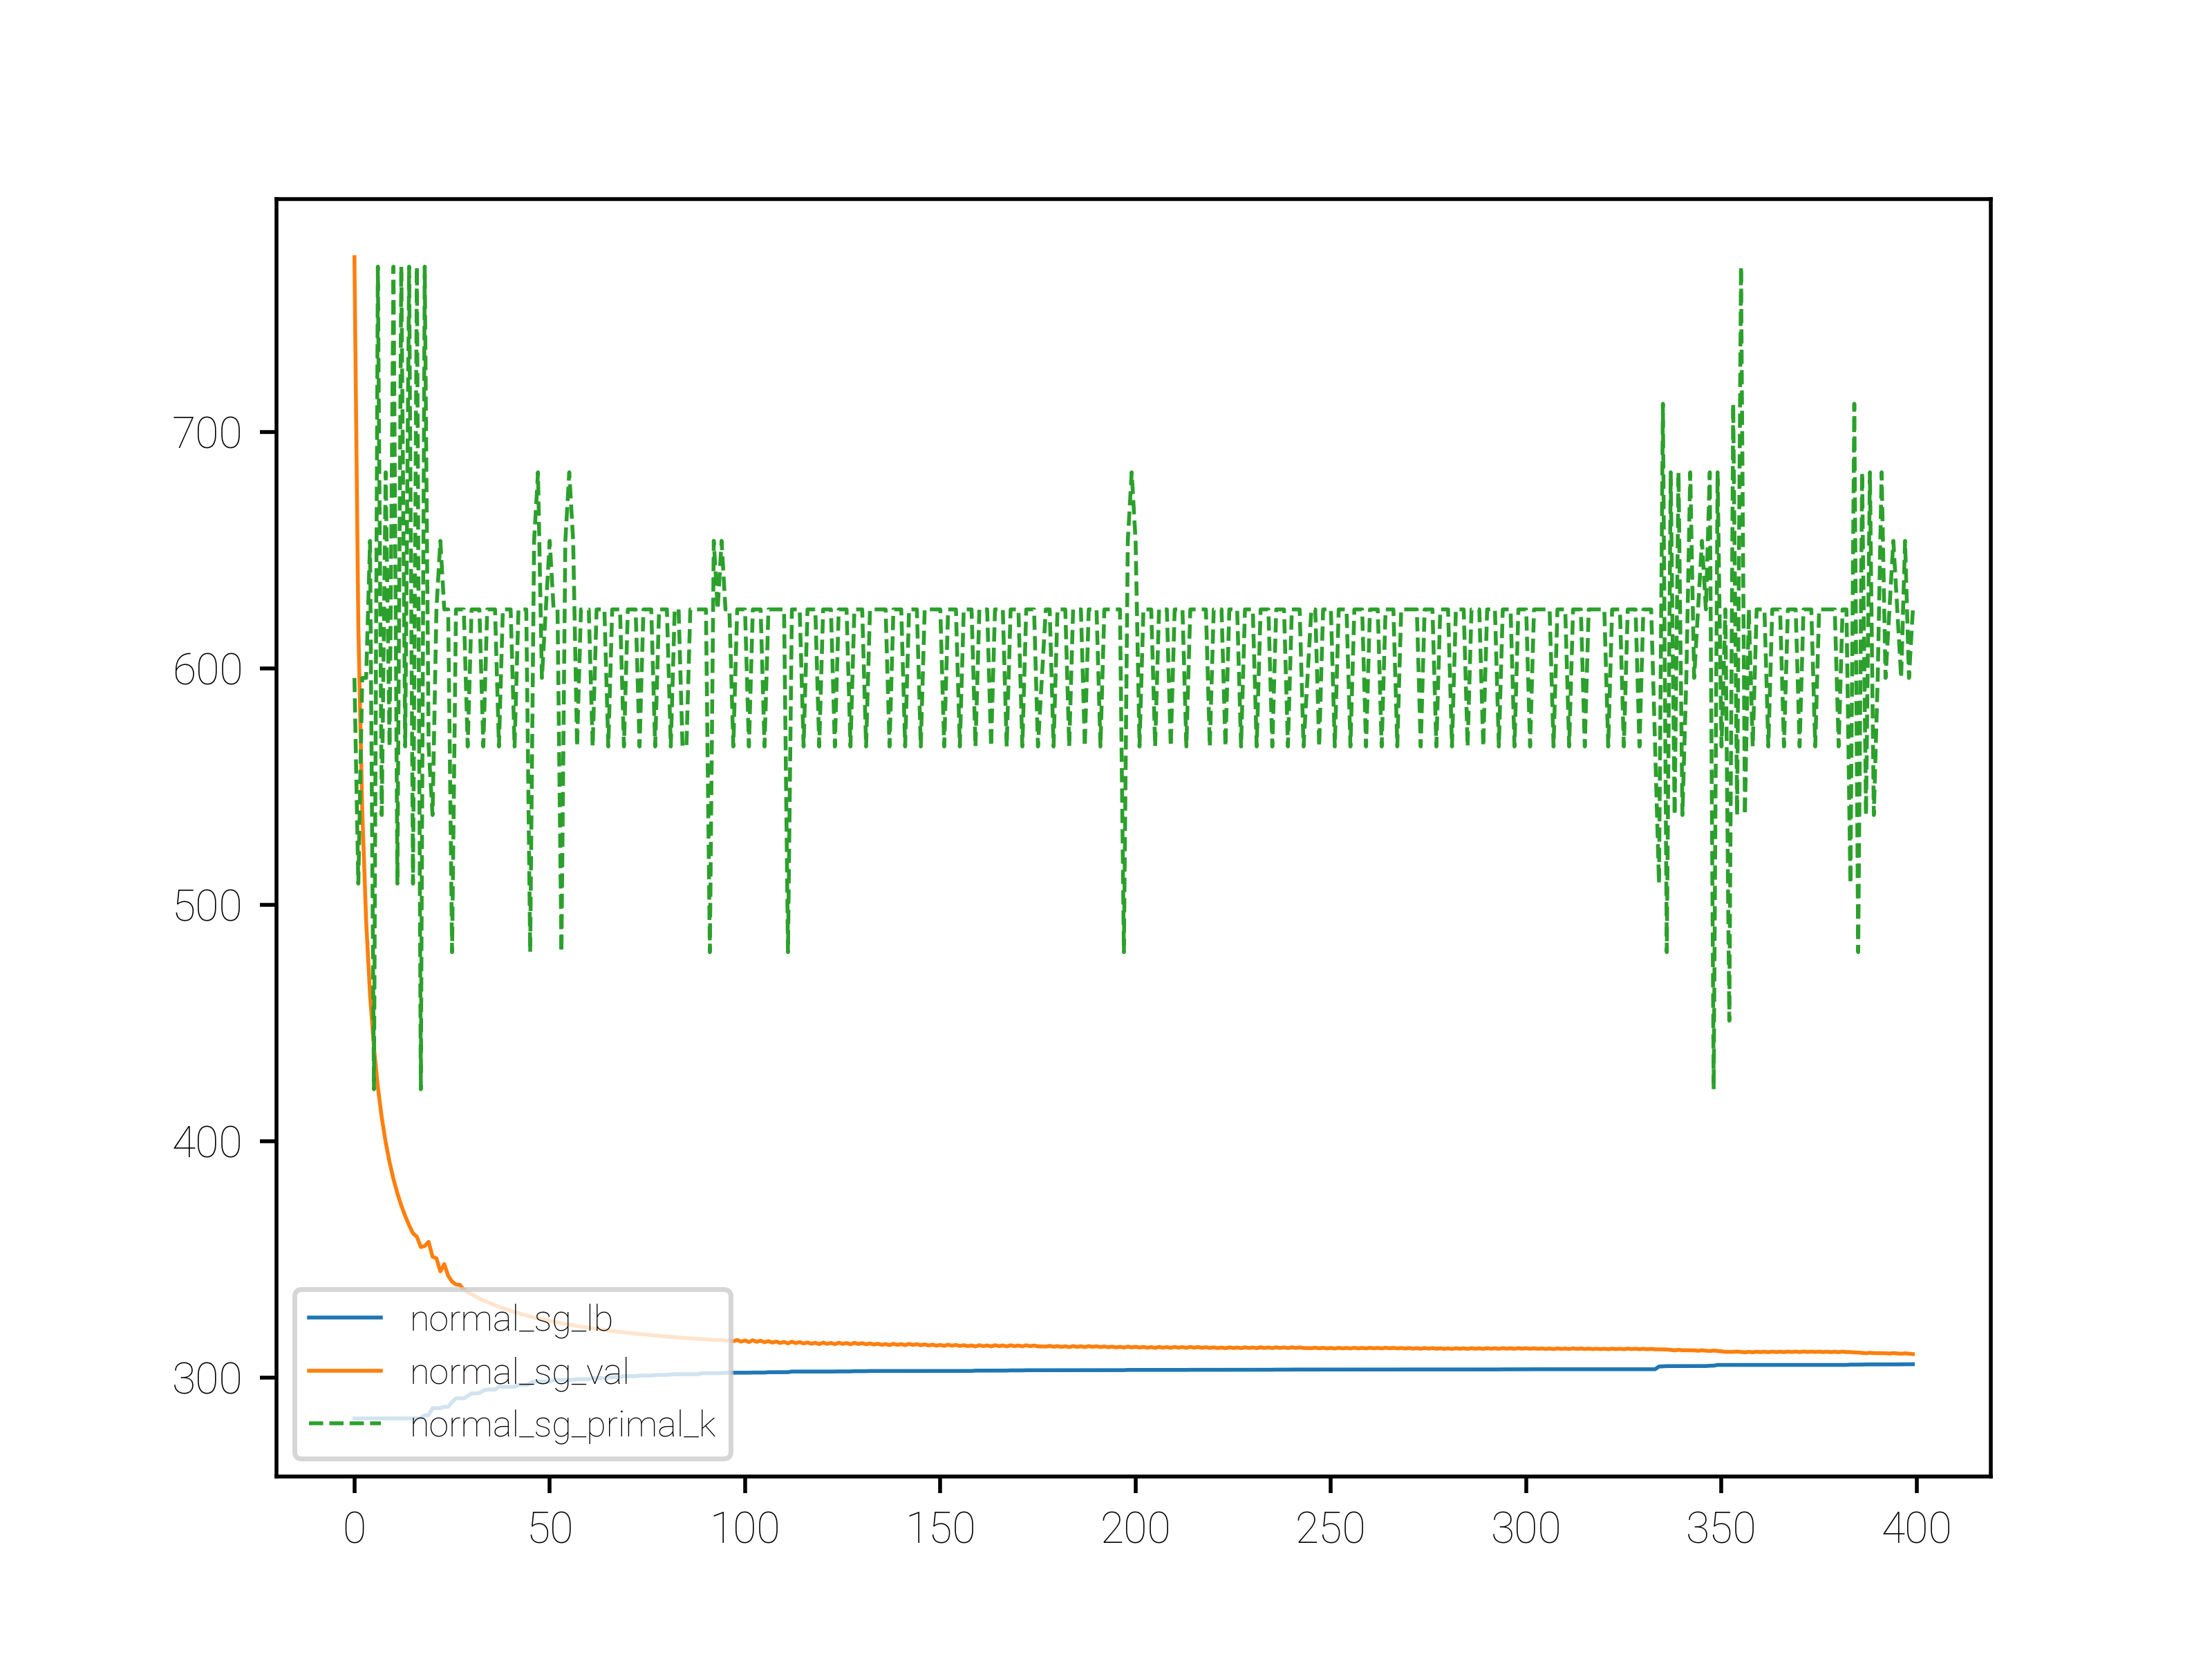
\includegraphics[width=.49\linewidth]{../imgs/conv_0_normal_sg_10_10.png}
  }
  \subfloat[][Convex subgradient method using \(d_k\)]{
    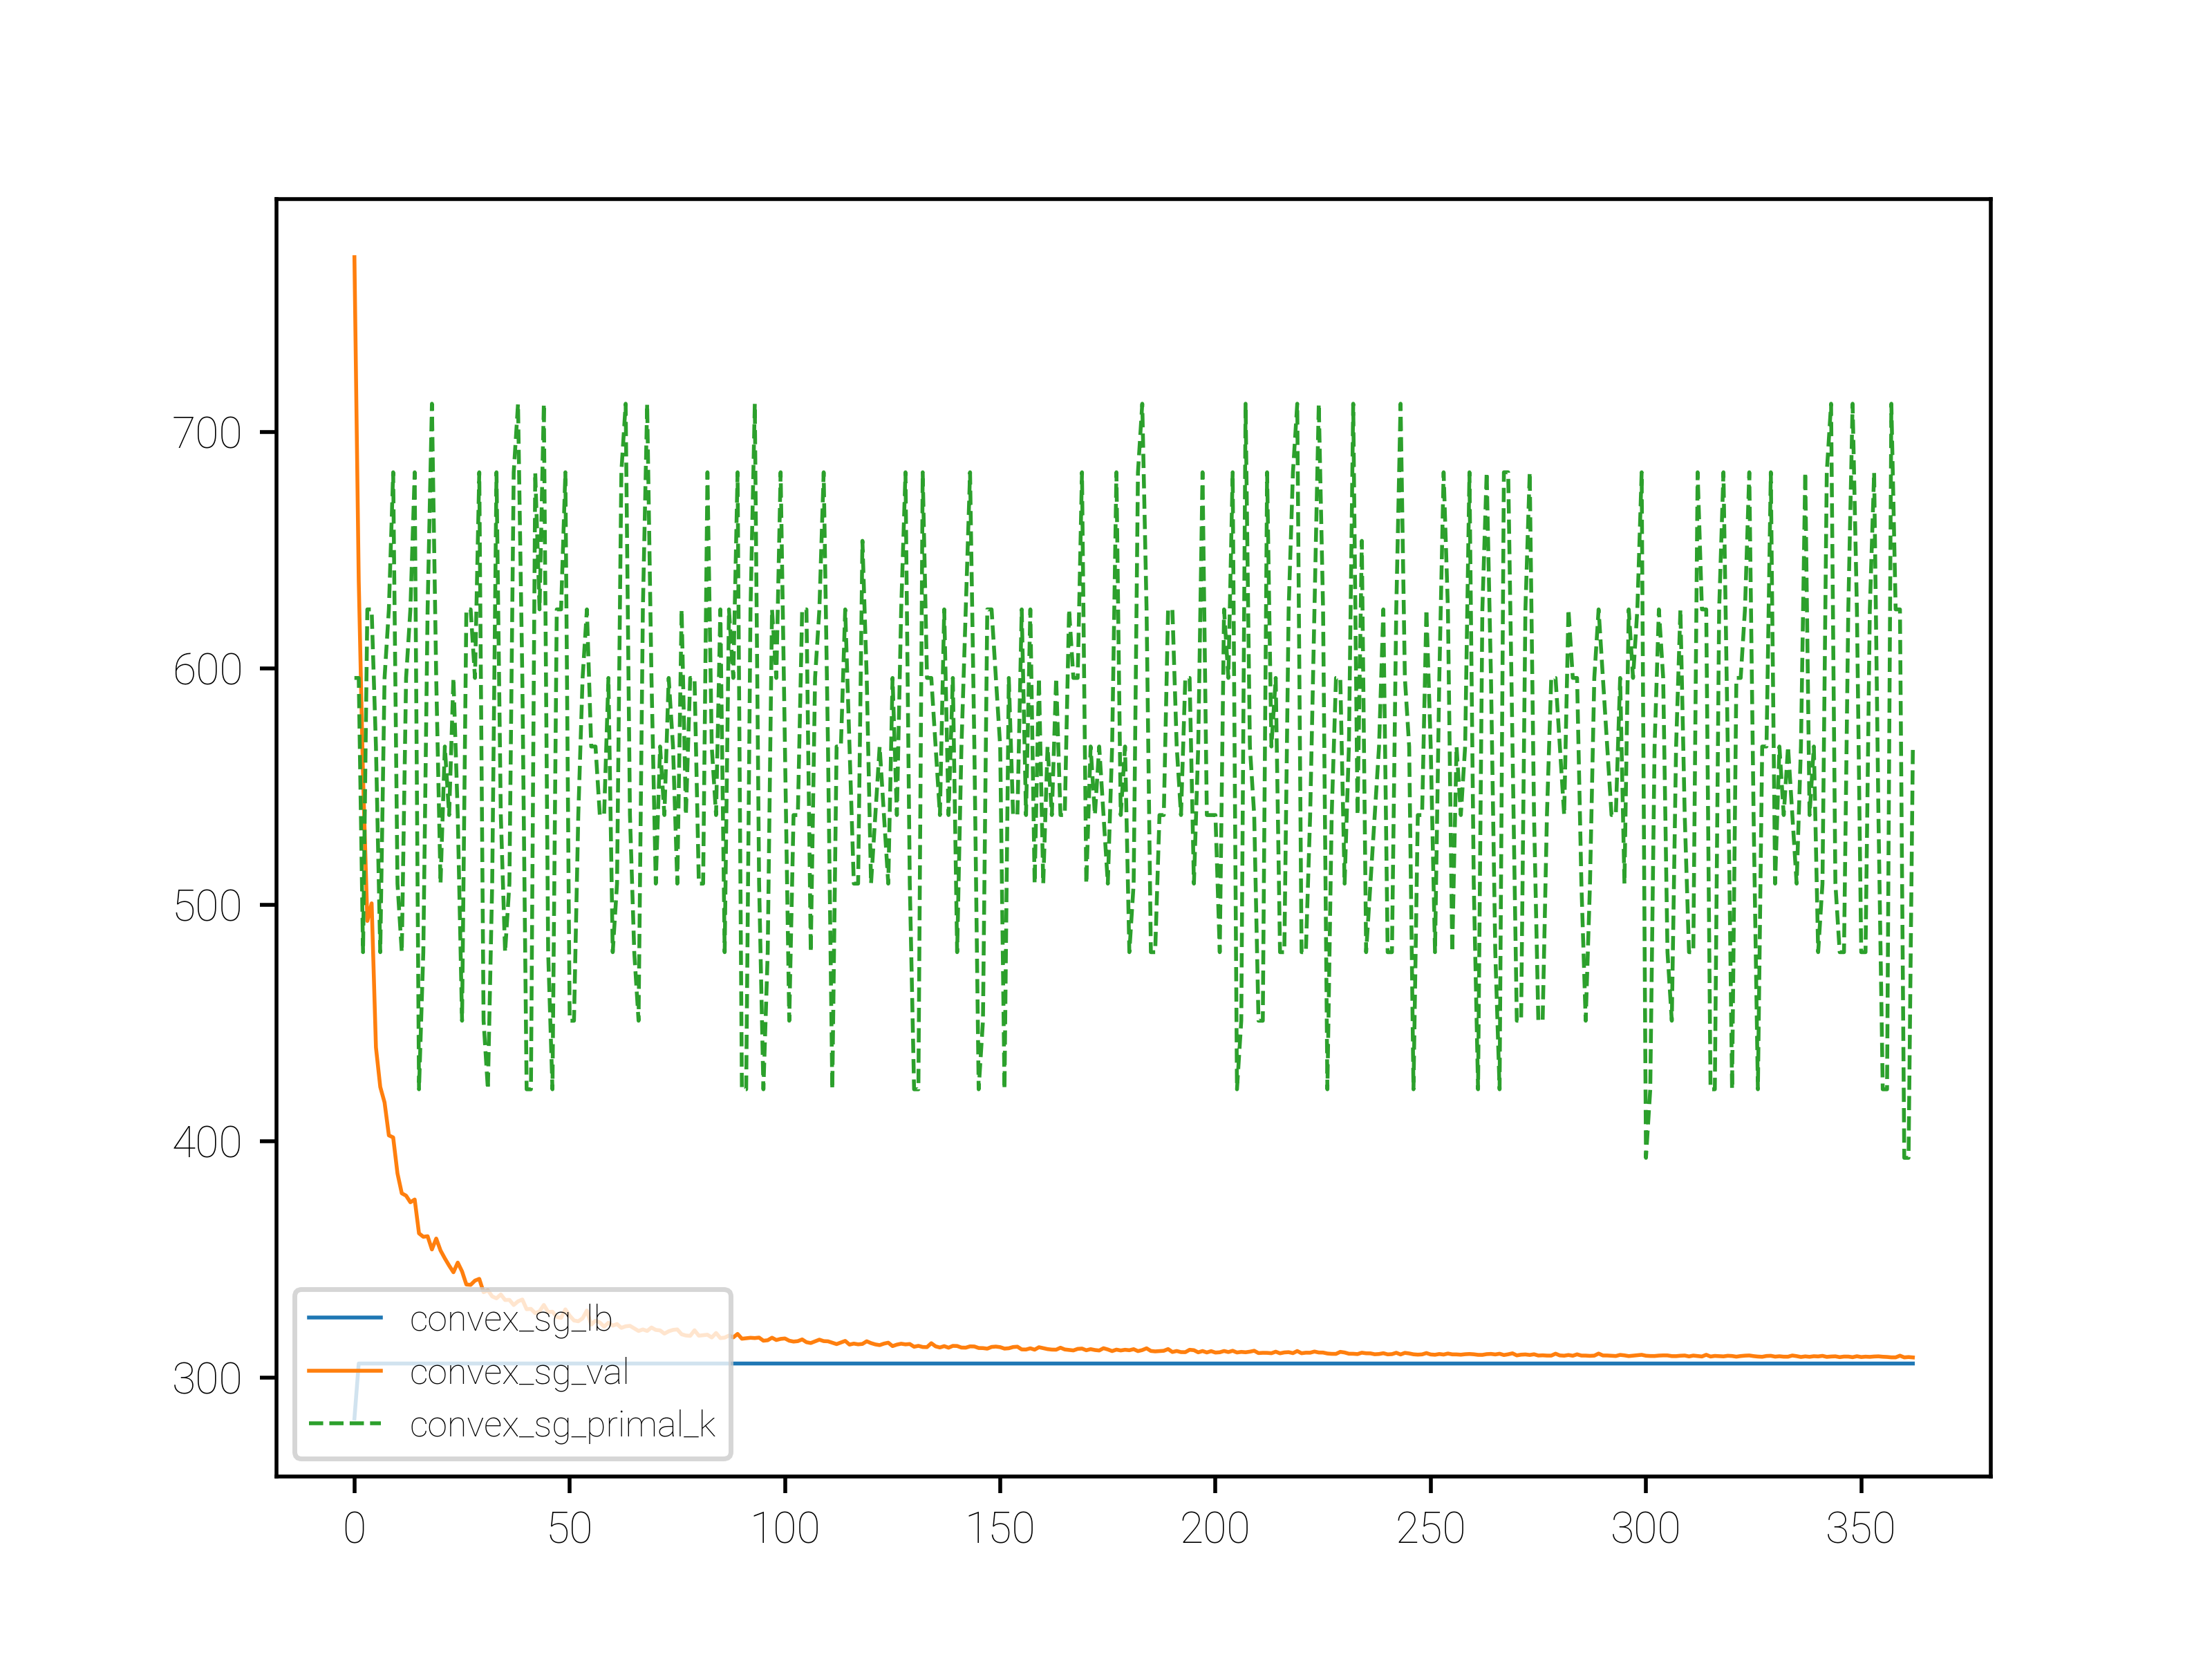
\includegraphics[width=.49\linewidth]{../imgs/conv_0_convex_sg_10_10.png}
  }

  \caption{
    An instance illustrating the convergence of the subgradient methods
    and the recovery algorithm \eqref{eq:recovery}.
    \textsf{sg\_lb} and \textsf{sb\_val}  are lower bound for the subgradient method
    and averaged primal value from the recovery algorithm, respectively.
    \textsf{primal\_k} is the primal value at iteration \(k\) without averaging.
  }

  \label{fig:divergent_volume}
\end{figure}


We summarize all test cases in Table \ref{tab:comp_repair_cases}.


\end{document}